
\documentclass[UTF8,                %字符编码
               table,               % 支持表格
               9pt,                %正文字号
               aspectratio=43]      %屏幕比例4:3-43,16:9-169,16:10-1610
               {beamer}
\usepackage{graphicx}
\usepackage{amssymb}
\usepackage{amssymb,amsmath, amsthm, amsfonts}
\usepackage{txfonts}
\usepackage{pgfpages}
\usepackage{tabularx,multicol,subfigure}
\usepackage{array,booktabs,textcomp}
\usepackage{fancybox}  % shadowbox
\usepackage{colortbl,xcolor}

\mode<presentation>
{
    \usetheme{CambridgeUS}
    \useinnertheme{circles}
%  \useoutertheme{infolines}
%    \useoutertheme{tree}
    \usecolortheme{default}

    \setbeamercovered{highly dynamic}

    \setbeameroption{notes on second screen}
}

%% Verbatim环境
\RequirePackage{natbib,fancyvrb,xcolor}
\RecustomVerbatimEnvironment{Verbatim}{Verbatim}{frame=leftline,numbers=left,
                                                 rulecolor=\color{lightgray},
                                                 framerule=4pt,numbersep=3pt}
\fvset{frame=leftline,numbers=left,rulecolor=\color{lightgray},framerule=4pt,numbersep=3pt}

%================================R书写环境声明==========================================%
\newcommand{\acronym}[1]{\textsc{#1}}
\newcommand{\class}[1]{~\mbox{\textsf{#1}}~}
\newcommand{\code}[1]{~\mbox{\texttt{#1}}~}
\newcommand{\pkg}[1]{{~\normalfont\fontseries{b}\selectfont #1}~}
\newcommand{\proglang}[1]{~\textsf{#1}~}
\renewcommand{\today}{\number\year 年 \number\month 月 \number\day 日}%重定义中文日期

\renewcommand\baselinestretch{1.3}  %% 全局控制行间距


\usepackage[boldfont,slantfont,CJKchecksingle]{xeCJK}
%\setCJKmainfont{文泉驿等宽正黑}
\setCJKmainfont{Microsoft YaHei}

\graphicspath{{pic/}}

\title[R语言数据挖掘应用]{\huge{R语言介绍及企业级数据挖掘应用}}

\author{刘思喆}
\titlegraphic{\includegraphics[scale = 0.25]{JD.jpg}}
\institute[京东商城]{数据部\\推荐系统}
\date{\today}


\AtBeginSection[]
{
\begin{frame}<beamer>
    \large{\textbf{目录}}
\textcolor[rgb]{0.50,0.00,0.00}{ \rule{\textwidth}{.7pt} }
  \scriptsize{推荐系统}
  \vspace{0mm}
\begin{columns}[c]
  \column{0.35\textwidth}
    \includegraphics[width = 0.9\textwidth]{JD_v.jpg}
  \column{0.5\textwidth}
  \renewcommand\baselinestretch{.8}
    \large{
    \tableofcontents[sectionstyle=show/shaded,hideallsubsections]}
  \renewcommand\baselinestretch{1}
    \vspace{3mm}
\textcolor[rgb]{0.50,0.00,0.00}{   \rule{\textwidth}{.7pt} }
\end{columns}
\end{frame}
}

\begin{document}

\maketitle

\section{R语言简介}

\frame{\frametitle{起源}
R 语言由新西兰奥克兰大学的 Ross Ihaka 和 Robert Gentleman 两人共同发明,其词法和语法分别源自 Scheme 和 S 语言,R语言一般认为是 S 语言(John Chambers, Bell Labs, 1972)的一种实现(方言)。
\begin{figure}
    \centering
  \includegraphics[width=0.4\textwidth]{ross-robert.jpg}\\
  \caption{1992年,Ross Ihaka 和 Robert Gentleman在奥克兰大学成为同事。为了方便教授初等统计课程,二人开发了一种语言;而他们名字的首字母都是R,于是 R便成为了这门语言的名称。}
\end{figure}
}

\frame{
\frametitle{R的大版本变化}
\begin{description}
  \item[1.0.0] 完整的、稳定的统计功能
  \item[2.0.0] 内存管理的增强,以及一些新特性的增加(Sweave)
  \item[3.0.0] 支持长对象(超过$2^{31}-1$)
\end{description}
}

\frame{\frametitle{里程碑}
  \scalebox{0.65}[0.65]{
\rowcolors[]{1}{blue!5}{blue!2}
\begin{tabular}{p{2.15cm}|p{2.4cm}|p{11.1cm}}
  \hline
  Version 0.0.0 & May 1995  &   JCGS paper submitted \\
  Version 0.16 & 1996 & This is the last alpha version developed primarily by Ihaka and Gentleman. Much of the basic functionality from the "White Book" (see S history) was implemented. \\
  Version 0.49 & Apr 23, 1997 & This is the oldest available source release, and compiles on a limited number of Unix-like platforms. CRAN is started on this date, with 3 mirrors that initially hosted 12 packages. Alpha versions of R for Microsoft Windows and Mac OS are made available shortly after this version. \\
  Version 0.60 & Dec 5, 1997 & R becomes an official part of the GNU Project. The code is hosted and maintained on CVS. \alert{Mailing lists(Apr),Core team(Aug)}\\
  Version 1.0.0 & Feb 29, 2000 & 2.8MB, Considered by its developers stable enough for production use. \\
  Version 1.4.0 &  & S4 methods are introduced and the first version for Mac OS X is made available soon after. \\
  Version 2.0.0 & Oct 4, 2004 &  10MB, Introduced lazy loading, which enables fast loading of data with minimal expense of system memory. \\
  Version 2.1.0 &  & Support for UTF-8 encoding, and the beginnings of internationalization and localization for different languages. \\
  Version 2.11.0 & Apr 22, 2010 & Support for Windows 64 bit systems. \\
  Version 2.13.0 & Apr 14, 2011 & Adding a new compiler function that allows speeding up functions by converting them to byte-code. \\
  Version 2.14.0 &  Oct 31, 2011 & 22MB, Added mandatory namespaces for packages. Added a new parallel package. \\
  Version 2.15.0 & Mar 30, 2012 & New load balancing functions. Improved serialization speed for long vectors. \\
  Version 3.0.0 & Apr 3, 2013 &  Support for numeric index values $2^{31}$ and larger on 64 bit systems. \\
  \hline
\end{tabular}
}
}

\frame{\frametitle{R 语言的前身 S 语言}
\begin{itemize}
  \item 1975-1976年,贝尔实验室统计研究部使用一套文档齐全的Fortran库做统计研究,简称为SCS(Statistical Computing Subroutines);
  \item 当时的商业统计软件采用的是批处理的方式,一次性输出问题的所有相关的信息,这在那个时代需要几个小时。
      而贝尔实验室的统计学家们需要交互式数据分析方式,并且商业软件不能对程序做任何修改,
      因此SCS在贝尔实验室非常受欢迎;
  \item 但使用SCS做统计分析时,需要大量的Fortran编程,花在编程上的时间有些得不偿失
      --\alert{统计分析不应该需要编写Fortran程序!}
  \item 为了同SCS进行交互,于是一套完整的语言系统S诞生了
  \item S 语言的理念,用它的发明者John Chambers的话说就是"to turn ideas into software, quickly and faithfully."
\end{itemize}
}

\begin{frame}{什么是 R}
\begin{itemize}
  \item R 是 `GNU S', 一个自由的、有效的、用于统计计算和绘图的语言和环境,它提供了广泛的统计分析和绘图技术:
      包括线性和非线性模型、统计检验、时间序列、分类、聚类等方法。
  \item \alert{我们更倾向于认为R是一个环境,在R环境里实现了很多经典的、现代的统计技术。}
\end{itemize}
\end{frame}

\begin{frame}{R的荣耀}
  \begin{enumerate}
    \item<1> The Statistical Computing and Graphics Award(ASA, 2010)
    \item<1> Data Analysts Captivated by R's Power(NYTimes, 2009)
    \item<1-2> ACM Software System Award(1998), John Chambers
  \end{enumerate}

      \begin{block}{The S System}
        \begin{itemize}
        \setlength{\itemsep}{-0.00cm}
          \item will forever alter the way people analyze, visualize, and manipulate data...
          \item is an elegant, widely accepted, and enduring software system, with conceptual integrity.
        \end{itemize}

        S is the one and only statistical system which is awarded by The ACM.
      \end{block}
\end{frame}

\begin{frame}
\frametitle{ACM Software System Award}
        \begin{itemize}
            \setlength{\itemsep}{-0.00cm}
          \item 1983 Unix
          \item 1986 TeX
          \item 1989 PostScript
          \item 1991 TCP/IP
          \item 1995 World-Wid-Web
          \item 1997 Tcl/Tk
          \item 1998 S
          \item 1999 The Apache Group
          \item 2002 Java
          \item 2009 VMware Workstation for Linux
          \item 2010 GroupLens Collaborative Filtering Recommender Systems
          \item 2011 Eclipse
          \item 2012 LLVM
        \end{itemize}
\end{frame}

\begin{frame}{现代数据分析理念}
  \begin{quotation}
    Can one be a good data analyst without being a half-good programmer?

    The short answer to that is, `No'.

    The long answer to that is, `No!'.

    -- Frank Harrell

    1999 S-PLUS User Conference, New Orleans
  \end{quotation}

R balances the current, partly conflicting needs of data analysts
and software developers in a near-optimal way (Bill Venables).
\begin{itemize}
  \item interactive flexibility vs code efficiency
  \item informal vs formal programming
\end{itemize}
\end{frame}

\section{应用现状}

\begin{frame}
  \frametitle{R或S的沿革}

  最近一两年开始被程序员社区关注
  \begin{itemize}
          \item 1984 interactive
          \item 1988 programming, S3
          \item 1991 statistics
          \item 1998 data, programming, S4
          \item 2008 software, data
  \end{itemize}
\end{frame}

\begin{frame}
    \frametitle{2012年KDnuggets网站关于数据挖掘软件的调查}
    \begin{figure}
      \centering
      \includegraphics[width = 0.6\textwidth]{kn.jpg}\\
      \caption{第13期KDnuggets 关于数据挖掘软件使用的调查-- 对于过去的12个月里实际的项目过程中使用了哪些数据挖掘(分析)软件,R、Excel和RapidMiner则名列三甲(去年R 排名第二)。另一份关于最常使用的底层语言依次为R语言、SQL、Java 和Python。}
    \end{figure}
\end{frame}

\begin{frame}
  \frametitle{商业软件对R的支持}
  \begin{itemize}
    \item Oracle, Oracle R Enterprise
    \item IBM Netezza, IBM InfoSphere BigInsights
    \item SAP HANA, Business Objects Predictive Analysis
    \item Teradata, teradataR
    \item Sybase RAP
    \item SAS
    \item PASW
    \item ...
  \end{itemize}
\end{frame}

\begin{frame}
  \frametitle{The solutions to Big Data}
  \begin{description}
    \item[Solution 1:]<1,2> Use R in Conjunction with other specialized tools(e.g MapReduce style tools, Hadoop, Streaming, Hive, Pig, Cascading...)
        \begin{description}
          \item[R + Hadoop] rhbase, rmr, rhdfs, RHIPE
          \item[R + MongoDB] RMongo, rmongodb
          \item[Segue] Amazon's Web Services(EC2)。
        \end{description}
    \item[Solution 2:]<1> Packages that enable new functionality for reading and processing very large data sets. (e.g bigmemory, ff, Enhance function, but no enhancements to the core language)
        \begin{description}
          \item[ff] offers file-based access to data sets that are too large to be loaded into memory
          \item[biglars] can use the ff to support large-than-memory datasets for least-angle regression, lasso and stepwise regression.
          \item[bigrf] a Random Forests implementation with support for parellel execution and large memory.
        \end{description}
  \end{description}
\end{frame}

\frame{\frametitle{Facebook}
    \begin{figure}
        \centering
\includegraphics[width = \textwidth]{facebook.png}
    \end{figure}
资料来源:\url{http://paulbutler.org/archives/visualizing-facebook-friends/}
}

\section{技术架构及支撑领域}

    \subsection{典型工作流}

\begin{frame}
  \frametitle{一般工作流程}
  \begin{enumerate}
    \item 通过Hive集群获取目标数据
    \item 在R环境下进行数据预处理
    \item R环境下分析建模(Featrue Selection, Benchmark)
    \item 评估(离线评估和分流量测试)
    \item 线上集成(R, Hive QL, Java, C++, Python...)
  \end{enumerate}
\end{frame}

\begin{frame}{数据的流动}
\begin{figure}
\centering
  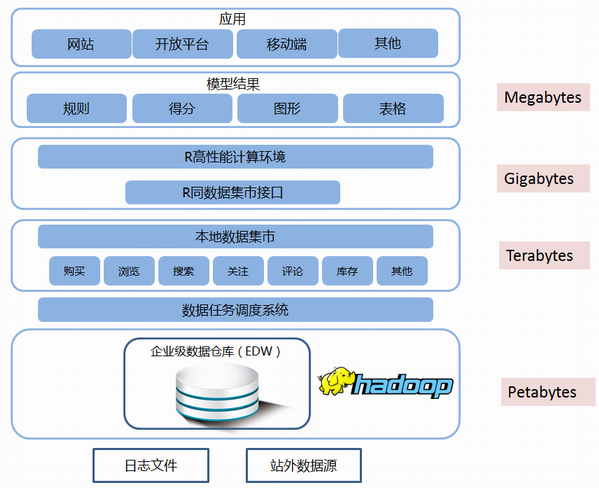
\includegraphics[height = 0.83\textheight]{Rdata.png}
\end{figure}
\end{frame}


    \subsection{涉及技术}
\begin{frame}
  \frametitle{涉及数据挖掘技术和相关的R包}
    \begin{itemize}
      \item 数据传递及服务(RHive、RServe、rJava)
      \item 清洗及预处理(sqldf、stringr、XML)
      \item 抽样、预测、分类、关联规则、特征选择、稀疏矩阵运算、矩阵分解、社交网络、分词、社交网络
      \item 高性能计算(rhdfs、rmr2、Rcpp)
      \item 其他
    \end{itemize}
\end{frame}



\begin{frame}
  \frametitle{挖掘模型服务对象}
  \begin{itemize}
    \item 在线广告优化
    \item 在线商品推荐
    \item 搜索词优化
    \item 邮件营销
    \item 移动客户端
    \item 活动及促销推送
    \item 开放平台的PoP商户
    \item ...
  \end{itemize}
\end{frame}

\section{案例}

\begin{frame}
  \frametitle{Case 1}
\begin{description}
  \item[用户A:] 男性、28岁、北京、累计购买金额13428元、没有投诉记录、最近2个月购买过ipad4 MD513CH,购买过图书三体,搜索过莫言、剃须刀、HDMI 转接线、手机等关键词,关注Sony KDL-46HX750 3D LED液晶电视,促销偏好度高……
  \item[用户B:] 女性、33岁、上海、累计购买金额3420元、曾有过投诉记录,记录关键词为安装慢、退货等,近2个月购买过ONLY圆领立体剪裁无袖修身连衣裙E(黑),蓝月亮亮白增艳自然清香洗衣液3000g,关注飞利浦 PT720 三刀头电动剃须刀,搜索过雅培、多美滋,促销偏好度低……
  \item[用户C:] ...
\end{description}

\pause
\alert{京东商城要做母婴专场活动,请问上述哪个用户更可能是目标客户群。}
\end{frame}

\begin{frame}
  \frametitle{模型的线下测试效果}
  \begin{itemize}
    \item 涉及用户数:9832608
    \item 购买概率大于0.34用户数:303641
    \item 未来5天实际购买用户数:14290
    \item 预测命中用户数:10337
  \end{itemize}

  \pause
  \begin{description}
    \item[对用户:] 最小程度地打扰客户,\alert{提高客户体验}
    \item[对企业:] 减低营销成本,提高客户忠诚度
  \end{description}
\end{frame}

\begin{frame}
  \frametitle{Case 2}
    逻辑回归的自动化实施
\end{frame}

\begin{frame}
  \frametitle{Case 3}
  获取商品详情页的信息
\end{frame}

\begin{frame}
  \frametitle{部分应用案例}
  \begin{itemize}
    \item 基于京东评论的新词识别模型
    \item 商品的价格弹性模型
    \item 商品性别色彩模型
    \item 京东商城“不良”商品识别模型
    \item PoP商家分群模型
    \item 京东商城三级类目购买关系模型
    \item 某品类评论关键词网络模型
    \item 商品销量预测模型
    \item 促销活动兴趣度模型
    \item \alert{潜在用户识别模型(用于定向营销)}
    \item 搜索桥梁词识别
  \end{itemize}
\end{frame}

\begin{frame}
\begin{center}
  \Huge{Q \& A}
\end{center}

\vspace{1cm}
  \begin{itemize}
     \item 邮件:\href{mailto:sunbjt@gmail.com}{liusizhe\textless at\textgreater jd.com}
     \item 博客 : \url{http://www.bjt.name}
     \item 微博:@刘思喆
  \end{itemize}
\begin{flushright}
\hyperlink{Return}{\beamerbutton{Jump to first slide}}
\end{flushright}

\end{frame}
\note{Talk no more than 1 minute.}



\end{document}


